\documentclass{article}
\usepackage{amsmath, amssymb, amsthm, graphicx}

\title{Chapter 2 Section 1}
\author{Andrew Taylor}
\date{March 26 2022}
\newtheorem{theorem}{Theorem}
\newtheorem{problem}{Problem}
\newtheorem*{solution}{Solution}

\begin{document}
\maketitle

\begin{problem}
Imagine yourself cruising in the Mediterranean as a crew member on a French coast goard boat, looking for evildoers. Periodically, your boat radios its position to headquarters in Marseille. You expect that communications will be intercepted. So, before you broadcast anything, you have to transform the actual position of the boat,

\begin{align*}
\begin{bmatrix}
x1 \\ x2
\end{bmatrix}
\end{align*}

($x_{1}$ for Eastern longitude, $x_{2}$ for Northern latitude), into an encoded position

\begin{align*}
\begin{bmatrix}
y_{1} \\ y_{2}
\end{bmatrix}
\end{align*}

You use the following code:

\begin{align*}
y_{1} &= x_{1} + 3x_{2} \\
y_{2} &= 2x_{2} + 5x_{2}
\end{align*}

For example, when the actual position of your boat is $5^\circ E$, $42^\circ N$, or

\begin{align*}
\vec{x} = \begin{bmatrix} x_{1} \\ x_{2} \end{bmatrix} = \begin{bmatrix} 5 \\ 42 \end{bmatrix}
\end{align*}

your encoded position will be 

\begin{align*}
\vec{y} 
&= \begin{bmatrix} y_{1} \\ y_{2} \end{bmatrix} \\
&= \begin{bmatrix} 
x_{1} + 3x_{2} \\ 
2x_{1} + 5x_{2} 
\end{bmatrix} \\
&= \begin{bmatrix}
5 + 3 * 42 \\ 2 * 5 + 5 * 42
\end{bmatrix} \\
&= \begin{bmatrix} 
131 \\ 220
\end{bmatrix}
\end{align*}

The coding transformation can be represented as

\begin{align*}
\vec{y} 
&= \begin{bmatrix} y_{1} \\ y_{2} \end{bmatrix} \\
&= \begin{bmatrix} 1 & 3 \\ 2 & 5  \end{bmatrix} \\
&= \begin{bmatrix} x_{1} \\ x_{2} \end{bmatrix}
\end{align*}

Figure 1

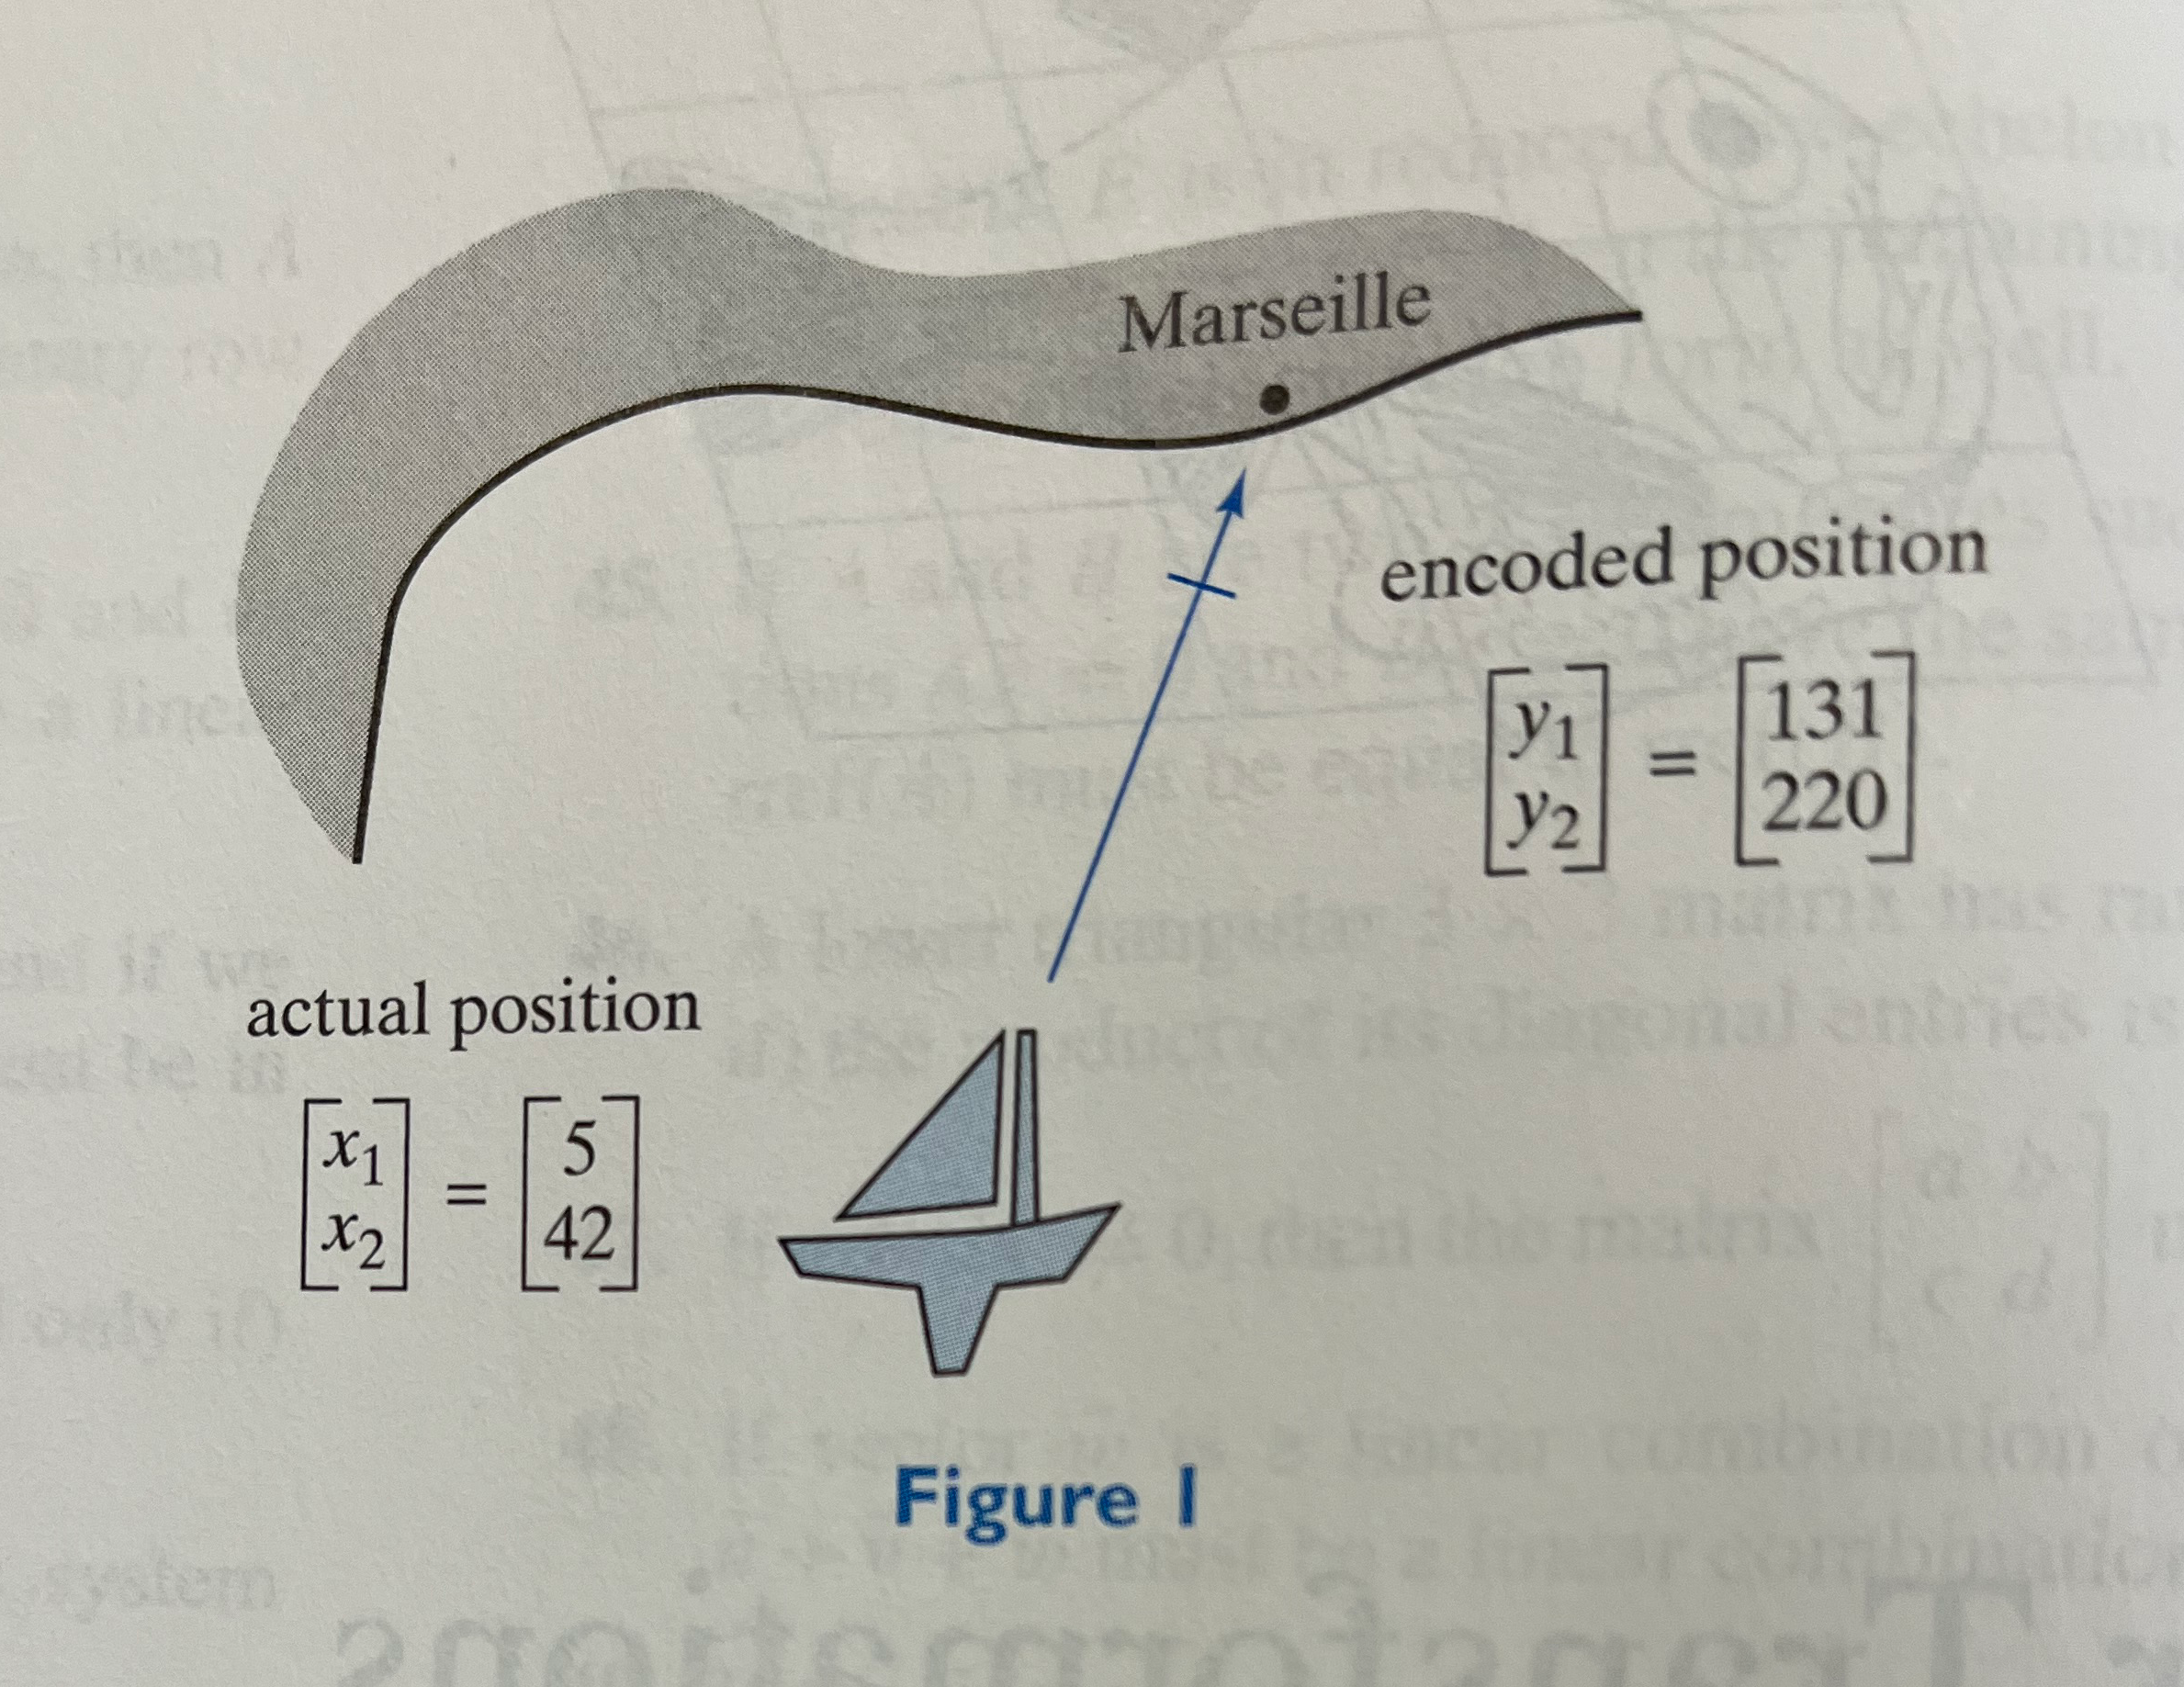
\includegraphics[scale=0.1]{ch2sec1fig1} 


As the ship reaches a new position, the sailor on duty at headquarters in Marseille receives the encoded message

\begin{align*}
\vec{b} = \begin{bmatrix} 133 \\ 223 \end{bmatrix} 
\end{align*}

He must determine the actual position of the boat. He will have to solve the linear system

\begin{align*}
A\vec{x} = \vec{b}
\end{align*}

or, more explicitly,

\begin{align*}
\begin{vmatrix}
x_{1} + 3x_{2} = 133 \\
2x_{1} + 5x_{2} = 223
\end{vmatrix}
\end{align*}

Here is his solution. Is it correct?

\begin{align*}
\vec{x} = \begin{bmatrix} x_{1} \\ x_{2} \end{bmatrix} = \begin{bmatrix} 4 \\ 43 \end{bmatrix}
\end{align*}

\end{problem}

\begin{solution}

We can use elementary row operations to solve the system. Remember, the elementary row operations are subtracting a multiple of a row, dividing a row by a scalar, and swapping rows.

\begin{align*}
& \begin{bmatrix}
1 & 3 & 133 \\
2 & 5 & 223
\end{bmatrix} \\
&\begin{bmatrix}
1 & 3 & 133 \\
0 & -1 & -43
\end{bmatrix} \\
& \begin{bmatrix}
1 & 3 & 133 \\
0 & 1 & 43
\end{bmatrix} \\
& \begin{bmatrix}
1 & 0 & 4 \\
0 & 1 & 43
\end{bmatrix}
\end{align*}

Thus his solution is correct. The solution is 

\begin{align*}
\vec{x} = \begin{bmatrix} x_{1} \\ x_{2} \end{bmatrix} = \begin{bmatrix} 4 \\ 43 \end{bmatrix}
\end{align*}

\end{solution}

\end{document}